\documentclass[11pt]{article}
\usepackage[review]{acl}
\usepackage{times}
\usepackage{latexsym}
\usepackage[T1]{fontenc}
\usepackage[utf8]{inputenc}
\usepackage{microtype}
\usepackage{inconsolata}
\usepackage{graphicx}
\usepackage{booktabs,longtable,amsmath,amssymb,enumitem}

\newcommand{\vx}{\mathbf{x}}
\newcommand{\vq}{\mathbf{q}}
\newcommand{\vd}{\mathbf{d}}
\newcommand{\vmu}{\boldsymbol{\mu}}
\newcommand{\R}{\mathbb{R}}

\title{Compressed Embeddings Fail Unevenly Across Languages,\\and Removing the Mean Fixes Most of It}

\author{Anonymous}

\begin{document}
\maketitle

\begin{abstract}
On-device search stores embedding vectors at 1--8 bits per dimension, and the evidence that this is cheap comes from English. We measure the retrieval loss of six storage formats in 122 languages with parallel content (Belebele) for five multilingual embedding models, and on a task with 28 times more passages. At 8 and 4 bits the average loss is under 2\%. Below that, the loss is uneven in every model, smallest for English and largest for low-resource languages, and its size depends on the model: under 1-bit storage, language groups lose 7--71\% of nDCG@10 with multilingual-E5 but under 5\% with BGE-M3 and Qwen3-Embedding. Within a model, the float32 margin between the relevant document and the strongest distractor orders the languages (Spearman $\rho$ from $-0.81$ to $-0.98$); across models, the loss grows with anisotropy. Removing the mean stepwise, with the model fixed, widens margins faster than compression noise, lowering the loss at each step. Calibration is not the cause: other languages or unrelated English text change group losses by 4 points at most. Subtracting an English mean vector from documents and queries cuts the E5 1-bit loss to under 4\% in every language group, below product quantization at equal storage.
\end{abstract}

\section{Introduction}
Dense retrieval represents every document as a vector and answers a query by finding the documents whose vectors score highest against the query's vector. On a phone or a laptop the vectors of the whole corpus sit in memory, so they are stored at reduced precision: float16 or int8 by default, and 4, 2 or 1 bit per dimension when memory is tight \citep{shakir2024quant,yamada2021bpr}. Recent measurements say this is nearly free: float8 loses under 0.3\% of retrieval quality on the Massive Text Embedding Benchmark (MTEB; \citealp{muennighoff2023mteb,sanchez2025storage}), and combined with dimensionality reduction, embeddings shrink to a fraction of a percent of their size with little loss \citep{dimquant2026}. Both measurements use English models on English data, and \citet{dimquant2026} name other languages as an open question.

Multilingual embedding models serve many languages that they handle less well than English. Compressing weights is known to hurt low-resource languages more than English in translation and generation \citep{ahia2021doublebind,marchisio2024quantization,mekala2025longcontext}. Whether compressing the \emph{stored embeddings} does the same, and why, has not been measured. We ask three questions. Does compression cost some languages more than others? If so, is the cause the \emph{calibration data}, since integer formats need a number range per dimension and practitioners estimate it on English text? And if not, what is the cause, and what removes it? We answer them on a benchmark whose content is identical in all 122 languages, so that a difference between two languages is a difference in how the model embeds them, not in the task, and check the answers on a second task with much larger corpora.

\paragraph{Findings.}
\begin{enumerate}[nosep,leftmargin=*]
\item \textbf{The loss is uneven in every model, and its size is the model's.} Below 4 bits, English loses least and low-resource languages most in all five models. Under 1-bit storage the E5 models lose 7--71\% and BGE-M3 and Qwen3 1--4\% by language group, even at equal dimensionality (\S\ref{sec:uneven}).
\item \textbf{Two float32 statistics account for most of the loss.} Within a model, the score margin orders the languages ($\rho$ from $-0.81$ to $-0.98$); across models, the loss grows with anisotropy, and the two explain 76\% of its variance over 610 model--language pairs. Removing the mean in steps, with the model fixed, widens margins 4.2-fold but compression noise only 1.6-fold, and the loss falls at every step (\S\ref{sec:whiten}).
\item \textbf{The calibration language is not the cause; the range estimator is.} Other calibration languages, or English text unrelated to the benchmark, change group losses by about 4 points at most; percentile clipping halves the 2-bit loss (\S\ref{sec:calib}).
\item \textbf{Subtracting the mean from documents and queries removes most of the loss}, with one vector fitted on as few as 16 English texts; centering only one side does not. At 1 bit per dimension it beats product quantization and PCA at equal storage; without it, product quantization keeps the inequality (\S\ref{sec:whiten}, \S\ref{sec:matched}). Model ordering and fix both hold on 28 times larger corpora (\S\ref{sec:wiki}).
\end{enumerate}
Code and per-language results are released.\footnote{\url{https://anonymous.4open.science/r/embedding-compression-languages-23FB}}

\section{Related Work}
\paragraph{Embedding compression.} Product quantization \citep{jegou2011pq} and its descendants in Faiss \citep{johnson2019faiss} compress vectors with learned codebooks. We study the simpler scalar formats that on-device libraries and vector databases expose directly: per-dimension integer quantization and sign binarization, popularized for sentence embeddings together with a float rescoring step by \citet{shakir2024quant}, and binary passage retrieval \citep{yamada2021bpr}. Matryoshka representations \citep{kusupati2022matryoshka} reduce the number of dimensions rather than their precision. \citet{sanchez2025storage} and \citet{dimquant2026} evaluate scalar formats and dimensionality reduction on English MTEB tasks. We extend the measurement to 122 languages and ask what predicts the per-language loss.

\paragraph{Compression and the long tail.} Pruning and quantizing model \emph{weights} damages rare inputs and low-resource languages more than frequent ones \citep{hooker2020bias,ahia2021doublebind}, with exceptions under some sparsification regimes \citep{ogueji2022intriguing}. For multilingual LLMs, weight quantization hurts non-English and non-Latin-script languages more than English \citep{marchisio2024quantization,mekala2025longcontext}, with calibration on 128 English samples throughout. We study a different object, the stored embedding, find the same direction of inequality, test the calibration-language explanation directly, and identify a per-language statistic that tracks the damage.

\paragraph{Anisotropy and centering.} Contextual embeddings occupy a narrow cone \citep{ethayarajh2019contextual,gao2019representation}, also in multilingual encoders, where the degree of anisotropy differs by language \citep{rajaee2022isotropy,hammerl2023anisotropy}. Removing the mean, and sometimes the top principal directions, is an established post-processing step for word and sentence embeddings \citep{mu2018allbutthetop,li2020bertflow,su2021whitening}, and binary hashing centers data before taking signs \citep{gong2011itq}. We do not propose centering. We find that the loss grows with anisotropy across five models and is ordered by the score margin within each, that centering must be applied to documents and queries alike, and that a mean fitted on English suffices for all 122 languages.

\paragraph{Tokenizer fertility.} Subword tokens per word differ by language and predict downstream quality \citep{rust2021tokenizer}. We find that fertility predicts the compression loss too, but less well than the margin.

\section{Method and Setup}\label{sec:method}
\paragraph{Retrieval and loss.} Documents and queries have unit-norm embeddings $\vd_i,\vq\in\R^d$, scored by $\vq^\top\vd_i$. Every task has one relevant document per query; we report nDCG@10. For a language and a format, \emph{loss} is $(\mathrm{nDCG}_{32}-\mathrm{nDCG}_{b})/\mathrm{nDCG}_{32}$ in percent, relative to the float32 quality of the same model on the same language.

\paragraph{Storage formats.} All formats are applied post hoc to the float32 corpus vectors; in the main results the query stays float32, the on-device setting where the corpus is stored compressed and the query is embedded at search time (compressed queries: Appendix~\ref{app:sym}). \textbf{float16} and \textbf{float8} (E4M3) are direct casts. \textbf{int$b$}, $b\in\{8,4,2\}$, maps dimension $j$ to $2^b$ evenly spaced levels between bounds $[l_j,u_j]$, either the minimum and maximum over a calibration set $\mathcal{C}$ \citep{shakir2024quant} or its 5th and 95th percentiles (\textbf{clip}); values outside are clipped. \textbf{Binary} keeps $\mathrm{sign}(x_j-t_j)$ with $t_j=0$ (\textbf{sign}) or the calibration mean of dimension $j$ (\textbf{mean-threshold}, ``bin-mean-thr'' in tables; the query is unchanged). Scores use the dequantized corpus vector. For $d=1024$, a vector costs 4096 bytes at float32, 512 at int4, 256 at int2 and 128 at 1 bit.

\paragraph{Calibration sources.} Every calibrated format is run with five sets $\mathcal{C}$ of 1388 vectors unless stated: \textbf{English}; \textbf{mixed}, a uniform sample over the other 121 languages that always excludes the evaluated language; \textbf{Latin-only}, the same restricted to Latin-script languages; \textbf{target, 64}, 64 target-language texts; and \textbf{target, all}, an oracle of 1388 target-language texts. The English set and the target-all set consist of all 488 passages and 900 questions of that language, so they coincide with its evaluation data, and because Belebele is parallel, every calibration set contains translations of the evaluated passages. The Wikipedia task, whose content differs between languages, is the control for this (\S\ref{sec:wiki}).

\paragraph{Margin, anisotropy, covariates.} The margin of a query is the float32 score of the relevant document minus the highest score among the others. It is positive exactly when the relevant document ranks first, and its size is the score noise the ranking can absorb before it flips. It is a top-1 quantity, whereas nDCG@10 also credits ranks 2--10; we use it as a proxy. The margin of a language is its mean over queries. Anisotropy is measured as the mean cosine $\bar c$ between two unrelated passages of the corpus. Language covariates are tokenizer \textbf{fertility} (tokens per document relative to English for the same documents), \textbf{script} (Latin or not) and resource class \citep{joshi2020state}; classes 0--1, 47 of the 122 languages, are called \emph{low-resource}. Six languages appear both natively and romanized (Arabic, Bengali, Hindi, Nepali, Sinhala, Urdu).

\paragraph{Centering, whitening, rescoring.} We fit the \textbf{centering} transform, $\vx\mapsto\vx-\vmu$, and shrunk zero-phase component analysis (\textbf{ZCA}) whitening, $\vx\mapsto\Sigma^{-1/2}(\vx-\vmu)$ with $\Sigma\leftarrow0.9\Sigma+0.1\bar\lambda I$, once on English or on the mixed sample, and apply them to the corpus and queries of every language before quantization, re-normalizing afterwards. Because a transform changes float32 quality, loss is also reported relative to the original float32 quality. For \textbf{rescoring}, we retrieve $k\in\{10,20,50,100\}$ candidates with the compressed corpus and rescore them with the float32 query against an int8 copy of the corpus (binary plus int8 costs 9/32 of float32) or the float32 corpus.

\paragraph{Learned compression at equal storage.} At the storage of 1 bit per dimension ($d/8$ bytes per vector) we compare against \textbf{product quantization} (PQ; \citealp{jegou2011pq}) with $d/8$ sub-quantizers of 256 centroids each (Faiss; \citealp{johnson2019faiss}), PQ after the centering transform, and \textbf{PCA} to $d/8$ dimensions stored at int8. Each is fitted on the 1388 English calibration vectors, or on 10{,}000 vectors sampled over all languages, enough to train the PQ codebooks; the query stays float32. We also fit the centering mean on 16, 64 or 256 English texts (five random draws each).

\paragraph{Data and models.} The main task is Belebele retrieval in MTEB \citep{bandarkar2024belebele,enevoldsen2025mmteb}: 488 passages and 900 questions in 122 language variants that translate the same content; 73 use the Latin script and 49 one of 26 other script codes. The second is the multilingual Wikipedia retrieval task of MMTEB \citep{enevoldsen2025mmteb}: 16 languages, about 13{,}500 passages and 1{,}500 queries each, with different content per language. Models are multilingual-e5-small (118M parameters, $d$=384), -base (278M, 768) and -large (560M, 1024) \citep{wang2024me5}, called E5 below; BGE-M3 (568M, 1024) \citep{chen2024bgem3}; and Qwen3-Embedding-0.6B (596M, 1024) \citep{zhang2025qwen3emb}, with each model's documented prefixes. The three 1024-dimensional models separate dimensionality from model family.

\paragraph{Statistics.} Embeddings are computed once per model (Qwen3 in float16). Formats with fixed calibration are deterministic; the mixed, Latin-only and target-64 calibration samples are drawn once with a fixed seed, the centering sample-size experiment uses five random draws, and PQ codebook training is random (Appendix~\ref{app:repro}). The variation we report is across languages, and means are over languages. Standard errors over 122 languages are at most 1.7 points for binary, 0.8 for int2-clip and 0.2 for int4. Group differences are tested with permutation tests (10{,}000 permutations of languages), correlations come with bootstrap 95\% intervals (5{,}000 resamples of languages), and regressions are OLS over model--language pairs with standard errors clustered by language.

\section{Results}
\subsection{The loss is uneven; its size is the model's}\label{sec:uneven}
\begin{table*}[t]\centering\footnotesize
\begin{tabular}{llrrrrrr}
\toprule
model & languages & int8 & int4 & int2 & int2-clip & bin-sign & bin-mean-thr \\
\midrule
E5-small & English & 0.0 & 0.5 & 6.6 & 2.5 & 27.1 & 9.4 \\
 & all 122 & 0.2 & 1.9 & 29.3 & 15.0 & 58.8 & 41.7 \\
 & low-res. & 0.2 & 2.7 & 37.9 & 19.4 & 70.9 & 50.1 \\
E5-base & English & 0.0 & 0.0 & 3.6 & 1.9 & 7.8 & 7.2 \\
 & all 122 & 0.1 & 1.1 & 17.8 & 9.1 & 29.2 & 26.7 \\
 & low-res. & 0.2 & 1.5 & 24.6 & 12.8 & 40.2 & 35.7 \\
E5-large & English & 0.0 & 0.1 & 1.7 & 0.7 & 6.7 & 2.8 \\
 & all 122 & 0.1 & 0.7 & 13.3 & 6.4 & 27.1 & 21.5 \\
 & low-res. & 0.1 & 1.0 & 19.4 & 9.6 & 38.4 & 29.9 \\
BGE-M3 & English & 0.0 & 0.1 & 0.8 & 0.3 & 1.0 & 1.6 \\
 & all 122 & 0.0 & 0.1 & 2.7 & 1.1 & 3.2 & 4.0 \\
 & low-res. & -0.1 & 0.1 & 3.5 & 1.3 & 4.1 & 4.8 \\
Qwen3-0.6B & English & 0.1 & 0.0 & 0.6 & 0.5 & 0.9 & 1.0 \\
 & all 122 & 0.0 & 0.1 & 2.3 & 1.1 & 2.0 & 3.8 \\
 & low-res. & 0.0 & 0.1 & 2.8 & 1.4 & 2.6 & 4.9 \\
\bottomrule
\end{tabular}
\caption{Relative nDCG@10 loss (\%) w.r.t.\ float32. Corpus compressed, query float32; integer ranges and mean thresholds (bin-mean-thr) calibrated on English; bin-mean-thr leaves the query unchanged and is not the centering transform of \S\ref{sec:whiten}. low-res.\ = 47 languages of Joshi class 0--1.}\label{tab:drop}
\end{table*}
Table~\ref{tab:drop} gives the loss per model for English, all languages and low-resource languages. float16 is lossless (at most 0.2\% in any language). float8 and int8 cost under 0.6\% on average in every model, at most 7.7\% in a single language (Tibetan, on which the E5 models already fail at float32). int4 costs E5-small 1.9\% on average and 2.7\% on low-resource languages, the other models at most 1.1\% on average, and single languages up to 10\%. Per language, 1 bit keeps 95\% of float32 quality in 103 of 122 languages with BGE-M3, while E5-small needs 4 bits in 100 languages (Table~\ref{tab:bits} and Figure~\ref{fig:bits}, Appendix~\ref{app:figs}).

Below 4 bits the ordering English $<$ all languages $<$ low-resource holds in all five models and all formats, and is not driven by a few languages: under int2-clip, 99--100\% of the other 121 languages lose more than English for the E5 models and 80--86\% for BGE-M3 and Qwen3. Under binarization, the 47 low-resource languages lose more than the other 75 in every model (E5-small 70.9\% vs.\ 51.3\%, BGE-M3 4.1\% vs.\ 2.6\%, Qwen3 2.6\% vs.\ 1.7\%; permutation test, $p<0.002$ for every model). Defining low-resource languages instead as the 47 with the fewest Wikipedia articles gives equal or larger gaps, and the median and worst-case losses follow the means (Table~\ref{tab:dist}, Appendix~\ref{app:mech}). Excluding the 2--8 languages per model on which the model fails at float32 changes no entry of Table~\ref{tab:drop} by more than 1.5 points, and recall@10 gives the same picture (binary loss 48\%, 22\%, 20\%, 2\% and 2\% for the five models).

The magnitude, however, differs by an order of magnitude between models. Under sign binarization E5-small loses 27\% in English and 71\% on low-resource languages (romanized Sinhala, Jingpho, Guarani and Wolof 85--88\%); E5-base 8\% and 40\%; E5-large 7\% and 38\%; BGE-M3 1.0\% and 4.1\%; Qwen3 0.9\% and 2.6\%. The worst language for BGE-M3, romanized Urdu, loses 16\%, less than the best language for E5-small. E5-large has the dimensionality of BGE-M3 and Qwen3 and higher float32 quality than Qwen3, yet loses 8 to 14 times more than they do on average: neither dimensionality nor float32 quality separates the models.

\subsection{Margin orders languages; loss grows with anisotropy}\label{sec:margin}
\begin{figure*}[t]\centering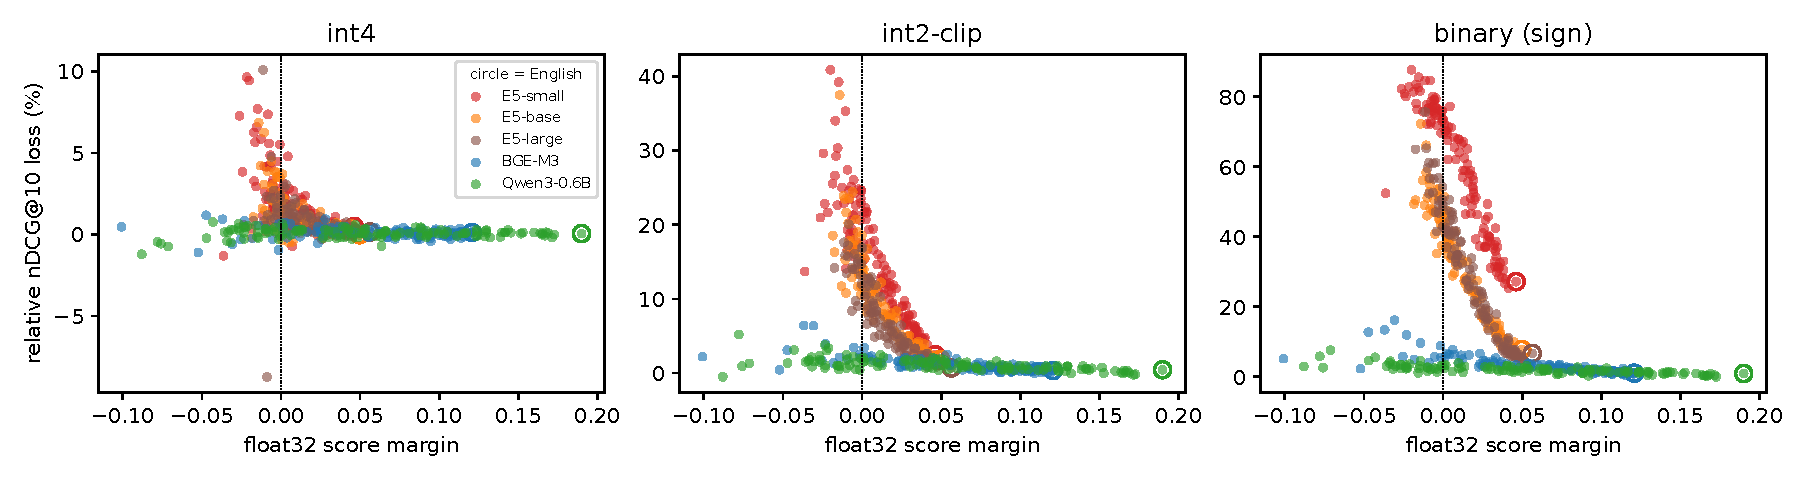
\includegraphics[width=\textwidth]{figs/fig1_loss_vs_margin.pdf}
\caption{Loss per language under int4, int2-clip and sign binarization (panels) against the language's mean float32 margin; one point per language and model, circles mark English. Under int2-clip and binarization the loss decreases with the margin within each model. Between models the curves differ: at the same margin, the anisotropic E5 models lose far more than BGE-M3 and Qwen3.}\label{fig:margin}\end{figure*}
\begin{table}[t]\centering\footnotesize
\setlength{\tabcolsep}{2pt}\begin{tabular}{lrrrrrrr}
\toprule
model & $d$ & nDCG & $\bar{c}$ & $\mu_{\mathrm{eng}}$ & $\mu_{\mathrm{low}}$ & $\rho_{\mathrm{bin}}$ & $\rho_{\mathrm{int2}}$ \\
\midrule
E5-small & 384 & 0.692 & 0.79 & 0.046 & -0.002 & -0.95 & -0.93 \\
E5-base & 768 & 0.736 & 0.78 & 0.050 & 0.003 & -0.98 & -0.96 \\
E5-large & 1024 & 0.785 & 0.77 & 0.056 & 0.008 & -0.98 & -0.96 \\
BGE-M3 & 1024 & 0.805 & 0.41 & 0.121 & 0.038 & -0.92 & -0.77 \\
Qwen3-0.6B & 1024 & 0.708 & 0.32 & 0.190 & 0.012 & -0.81 & -0.66 \\
\bottomrule
\end{tabular}
\caption{Embedding geometry per model. nDCG: float32 nDCG@10; $\bar{c}$: mean cosine between passages (mean over languages); $\mu$: mean float32 margin for English and for low-resource languages; $\rho$: Spearman correlation across the 122 languages between margin and loss under binarization / int2-clip.}\label{tab:geom}
\end{table}
\paragraph{Within a model, the margin orders the languages.} Figure~\ref{fig:margin} plots the loss of every language against its mean float32 margin. Within each model the loss decreases with the margin: Spearman $\rho$ between margin and binary loss is $-0.95$, $-0.98$, $-0.98$, $-0.92$ and $-0.81$ for E5-small, -base, -large, BGE-M3 and Qwen3 (Table~\ref{tab:geom}), and the bootstrap 95\% intervals exclude $-0.7$ for every model. Low-resource languages have the smallest margins in every model; for E5-small their mean margin is negative, so the relevant document often trails a distractor even at float32. The languages that a model embeds with thin margins are the same for every model (Spearman between the per-language margins of two models 0.90--0.98), and so are the per-language losses of the four encoder models (0.84--0.96; Qwen3, a decoder model, 0.57--0.70).

The float32 nDCG@10 of a language orders the languages almost as well as the margin ($\rho$ from $-0.80$ to $-0.97$), as it must, since both measure how far the relevant document is ahead of the distractors. We use the margin because it is the quantity the mechanism acts on, and because the two come apart under centering (\S\ref{sec:whiten}): centering raises the mean margin of E5-small fourfold while changing its float32 nDCG@10 by 6\%, and the binary loss falls from 59\% to 4\%.

\paragraph{Across models, the loss grows with anisotropy.} Figure~\ref{fig:margin} also shows that the margin alone does not explain the difference between models: at a margin of 0.05, an E5 language loses 5--27\% under binarization and a BGE-M3 or Qwen3 language under 4\%. Over the 610 model--language pairs, the margin alone explains 32\% of the variance of the binary loss ($R^2$); the margin with a model indicator explains 75\%. What distinguishes the models is anisotropy (Table~\ref{tab:geom}). In the E5 models two unrelated passages have mean cosine $\bar c$ of 0.77--0.79, so all scores share a narrow band and the English margin is 0.05--0.06; in BGE-M3 and Qwen3, $\bar c$ is 0.41 and 0.32 and the English margin 0.12 and 0.19. The margin, $\bar c$ and their interaction explain 76\% of the variance for binary and 71\% for int2-clip without any model identity. Anisotropic embeddings share a large common component. In the stored codes it makes most signs identical across documents and stretches the min/max ranges of integer formats; in an uncentered query it adds to every compressed score an offset that depends on the document but not on the query (\S\ref{sec:whiten}). Measured directly for E5-small, a query ranked first at float32 loses that rank under binarization in 94\% of cases when its margin is below a quarter of the perturbation of its scores and in 21\% when it exceeds twice the perturbation (Table~\ref{tab:flip}, Appendix~\ref{app:mech}). With five models this cross-model relation rests on five points and we treat it as descriptive; the within-model ordering is the result that 122 languages support.

\paragraph{Margin and language covariates.} Over the 575 pairs with a resource class, regressing the per-language loss on fertility, Latin script and resource class with model indicators gives $R^2=0.79$ for binary and $0.62$ for int2-clip, and fertility alone correlates with binary loss at $\rho=0.73$--$0.79$ for the encoder models (Figure~\ref{fig:fert}, Appendix~\ref{app:figs}). The margin, which needs no metadata about the language, explains nearly as much ($R^2=0.74$ and $0.57$ with model indicators). It does not absorb the covariates: with the margin in the model, resource class ($-4.6$ points of binary loss per class, $p<0.001$) and Latin script ($+3.8$ points, $p=0.004$) keep independent effects, and adding the three covariates raises $R^2$ to 0.79 and 0.62. Fertility adds nothing for binary ($p=0.11$) but does for int2-clip ($p=0.008$). The margin is therefore a metadata-free proxy for most, not all, of what the covariates capture.
Six languages make the point without any change of content (Table~\ref{tab:script}, Appendix~\ref{app:figs}). Romanizing the same Arabic, Bengali, Hindi, Nepali, Sinhala or Urdu text drives the E5 margin from $+0.01$--$0.03$ to between $-0.02$ and $-0.001$, the int2-clip loss from 4--10\% to 19--39\% and the binary loss from 21--47\% to 60--80\%: with identical content, romanization lowers the margin and raises the loss together.

\subsection{The calibration language does not matter; the estimator does}\label{sec:calib}
Table~\ref{tab:calib} isolates the calibration source on the three E5 models, the ones sensitive to it, and Table~\ref{tab:calib_full} has all five (both in Appendix~\ref{app:figs}). Replacing English calibration by the mixed sample, which never contains the evaluated language, or by Latin-script languages only, changes the pooled loss by at most 3.2 points in any row and the group-mean loss of any single model by at most 4.2 points, in both directions; single languages vary more. Even the in-language oracle, which has seen the evaluation vectors, recovers only a fifth to a third of the int2 and mean-threshold binary loss, so the calibration language explains little of the gap. Calibrating instead on English Wikipedia passages, which share no content with Belebele, changes the mean E5-small losses by at most 1.7 points (Table~\ref{tab:heldout}, Appendix~\ref{app:mech}).

Two estimator choices matter more. Clipping the range to the 5th--95th percentiles halves the mean and the low-resource int2 loss of every model (Table~\ref{tab:drop}: 29$\to$15\%, 18$\to$9\% and 13$\to$6\% for the E5 models): the min/max range is stretched by outliers, so most of the four int2 levels are spent on values that rarely occur. This is also why 64 in-language calibration vectors beat 1388 of them under min/max int2 (10\% vs.\ 16\%): a smaller sample has a narrower range. Second, setting each binary threshold at the calibration mean (mean-threshold, query unchanged) cuts the binary loss of E5-small from 27\% to 9\% in English and from 71\% to 50\% on low-resource languages; \S\ref{sec:whiten} shows why this is only half of the fix. Pooled over the E5 models, 64 target-language texts capture the in-language benefit of both fixes, and 1388 add at most 0.6 points.

\subsection{Subtracting the mean removes most of the loss}\label{sec:whiten}
\begin{table*}[t]\centering\footnotesize
\begin{tabular}{llrrrrrrrr}
\toprule
 & & & & \multicolumn{2}{c}{nDCG@10} & \multicolumn{3}{c}{binary loss (\%) vs.\ original float32} & vs.\ own float32 \\
\cmidrule(lr){5-6}\cmidrule(lr){7-9}\cmidrule(lr){10-10}
model & transform & $\bar{c}$ & margin & float32 & binary & all & low & int2-clip & binary, all \\
\midrule
E5-small & none & 0.79 & 0.010 & 0.692 & 0.318 & 58.8 & 70.9 & 15.0 & 58.8 \\
 & centered & 0.35 & 0.043 & 0.735 & 0.660 & 3.9 & 2.1 & -4.9 & 11.5 \\
\midrule
E5-base & none & 0.78 & 0.016 & 0.736 & 0.552 & 29.2 & 40.2 & 9.1 & 29.2 \\
 & centered & 0.34 & 0.054 & 0.764 & 0.719 & 2.6 & 3.0 & -2.8 & 7.0 \\
\midrule
E5-large & none & 0.77 & 0.021 & 0.785 & 0.604 & 27.1 & 38.4 & 6.4 & 27.1 \\
 & centered & 0.33 & 0.067 & 0.804 & 0.771 & 1.8 & 2.1 & -1.7 & 4.8 \\
\midrule
BGE-M3 & none & 0.41 & 0.064 & 0.805 & 0.783 & 3.2 & 4.1 & 1.1 & 3.2 \\
 & centered & 0.18 & 0.092 & 0.808 & 0.792 & 1.9 & 2.6 & 0.3 & 2.4 \\
\midrule
Qwen3-0.6B & none & 0.32 & 0.055 & 0.708 & 0.695 & 2.0 & 2.6 & 1.1 & 2.0 \\
 & centered & 0.13 & 0.071 & 0.713 & 0.703 & 0.6 & 0.7 & -0.3 & 1.5 \\
\bottomrule
\end{tabular}
\caption{Centering transform fitted on the English calibration mean and applied to documents and queries. $\bar{c}$: mean passage cosine; margin: mean float32 margin; nDCG@10: mean over 122 languages of the float32 quality after the transform and of the binary quality. Losses relative to the \emph{original} float32 quality mix two effects, the better float32 representation and the more robust compression; the last column, relative to the float32 quality after centering, isolates the second. Whitening and mixed-sample centering: Table~\ref{tab:whiten}.}\label{tab:centre}
\end{table*}

If the loss comes from a large common component, removing it should remove the loss. Table~\ref{tab:centre} and Figure~\ref{fig:fix} (left; Appendix~\ref{app:figs}) test this. Subtracting the calibration mean, one $d$-dimensional vector fitted on English and applied to the corpus and queries of all 122 languages, transforms the E5 models. For E5-small, $\bar c$ falls from 0.79 to 0.35, the mean margin rises from 0.010 to 0.043, float32 quality itself improves from 0.692 to 0.735, and the binary loss relative to the original float32 quality falls from 59\% to 3.9\% on average and from 71\% to 2.1\% on low-resource languages; int2-clip after centering is \emph{better} than the original float32. E5-base and E5-large follow (29$\to$2.6\% and 27$\to$1.8\%). Measured against the improved float32 baseline instead, the residual binary loss is 11.5\%, 7.0\% and 4.8\%, down from 59\%, 29\% and 27\%. Centering changes BGE-M3 and Qwen3 by under two points, because their spaces are already spread.

\paragraph{Both sides must be centered.} The centering transform stores exactly the codes of the mean-threshold format of \S\ref{sec:calib}, since re-normalizing does not change a sign; the two differ only in the query. For E5-small, centering only the stored vectors leaves a binary loss of 41.7\%, centering only the query 39.1\%, and centering both 3.9\% (low-resource languages: 50.1\%, 42.9\% and 2.1\%). Without centering, most signs are shared across documents and carry little information. With centered codes but an uncentered query, the common component $\vmu$ adds $\vmu^\top\mathbf{b}_i$ to the score of document $i$, an offset that varies between documents but not between queries and swamps thin margins. Removing the mean in steps holds the model fixed and varies only the geometry: as $\bar c$ falls from 0.79 to 0.35, the E5-small margin grows 4.2-fold, the score perturbation 1.6-fold, and the binary loss falls monotonically from 58.8\% to 3.9\% (Table~\ref{tab:graded}, Appendix~\ref{app:mech}).

 A mean fitted on the mixed sample is marginally better than the English one, so again the calibration language is secondary. Little data is needed for the mean: a mean of 16 English texts already brings the binary loss to 1.0--5.6\% across models (1388 texts: 0.6--3.9\%), with a standard deviation over five draws below 0.8 points. Full ZCA whitening fitted on 1388 English vectors overfits and lowers the float32 quality of every model (E5-small 0.692$\to$0.576); the common component, not the full covariance, carries the damage (Table~\ref{tab:whiten}, Appendix~\ref{app:figs}).

\paragraph{Rescoring helps less per byte.} Rescoring candidates against an int8 copy of the corpus (9/32 of float32) needs a number of candidates set by the model and the language (Figure~\ref{fig:fix} and Table~\ref{tab:rescore}, Appendix~\ref{app:figs}): 20 remove the binary loss of BGE-M3 and Qwen3, while 100 still leave E5-small 9\% on average and 13\% on low-resource languages (E5-base and -large: 2--3\%). At 1/32, centered binary loses less than rescoring with up to 50 candidates for every E5 model; with 100, rescoring is within a point of centering for E5-base and E5-large. We did not test rescoring on top of centering.

\subsection{Product quantization keeps the inequality}\label{sec:matched}
\begin{table*}[t]\centering\footnotesize
\begin{tabular}{lrrrrrrrrrr}
\toprule
 & \multicolumn{2}{c}{sign} & \multicolumn{2}{c}{centered sign} & \multicolumn{2}{c}{PQ} & \multicolumn{2}{c}{centered PQ} & \multicolumn{2}{c}{PCA + int8} \\
\cmidrule(lr){2-3} \cmidrule(lr){4-5} \cmidrule(lr){6-7} \cmidrule(lr){8-9} \cmidrule(lr){10-11}
model & all & low & all & low & all & low & all & low & all & low \\
\midrule
E5-small & 58.8 & 70.9 & 3.9 & 2.1 & 38.6 & 46.5 & 5.5 & 4.6 & 29.7 & 30.1 \\
E5-base & 29.2 & 40.2 & 2.6 & 3.0 & 23.0 & 30.9 & 2.3 & 2.1 & 9.7 & 9.7 \\
E5-large & 26.8 & 38.4 & 1.8 & 2.1 & 16.3 & 23.2 & 1.9 & 2.1 & 5.5 & 6.1 \\
BGE-M3 & 3.2 & 4.1 & 1.9 & 2.6 & 3.1 & 4.0 & 1.9 & 2.5 & 8.4 & 11.1 \\
Qwen3-0.6B & 2.0 & 2.6 & 0.6 & 0.7 & 2.5 & 3.3 & 0.9 & 1.0 & 8.6 & 11.1 \\
\bottomrule
\end{tabular}
\caption{Loss (\%) relative to the original float32 nDCG@10 at the storage of 1 bit per dimension ($d/8$ bytes per vector): sign binarization, sign after the centering transform (documents and queries), product quantization with $d/8$ 8-bit sub-quantizers (PQ), PQ after centering, and PCA to $d/8$ dimensions stored at int8. All fitted on 1388 English vectors; query float32. Computed on re-embedded vectors (Appendix~\ref{app:repro}).}\label{tab:matched}
\end{table*}

Product quantization learns its codebooks from data, so one might expect it to avoid the problem. It does not (Table~\ref{tab:matched}). At the storage of 1 bit per dimension, PQ fitted on English loses 4.8\% in English with E5-small but 38.6\% on average and 46.5\% on low-resource languages; E5-base and E5-large keep the same pattern (English 3.3\% and 1.8\%, low-resource 30.9\% and 23.2\%). Training the codebooks on 10{,}000 vectors from all languages instead changes the all-language loss by at most 2.5 points. PCA with int8 storage subtracts the mean as part of the projection; for the E5 models it loses about as much on low-resource languages as on average and less than PQ, but still 5.5--29.7\%, and it is the worst option for BGE-M3 and Qwen3 (8.4--8.6\%). Centering first fixes PQ as it fixes the sign: centered PQ loses 0.9--5.5\%, close to centered sign binarization (0.6--3.9\%), which needs no codebook. The cause is again the common component, and removing it matters more than the choice of quantizer.

\subsection{A second task with larger corpora}\label{sec:wiki}
\begin{table*}[t]\centering\footnotesize
\begin{tabular}{llrrrrrrr}
\toprule
model & task & nDCG & margin & int2-clip & bin-sign & bin-mean-thr & $\rho_{\mathrm{bin}}$ \\
\midrule
E5-small & Wikipedia & 0.877 & 0.025 & 3.4 & 27.1 & 18.8 & -0.54 \\
 & Belebele & 0.906 & 0.034 & 5.5 & 33.9 & 23.1 & -0.86 \\
E5-base & Wikipedia & 0.888 & 0.027 & 1.4 & 5.6 & 6.5 & -0.78 \\
 & Belebele & 0.927 & 0.039 & 3.0 & 10.8 & 11.2 & -0.69 \\
E5-large & Wikipedia & 0.908 & 0.031 & 0.8 & 3.1 & 3.9 & -0.60 \\
 & Belebele & 0.948 & 0.044 & 1.8 & 7.7 & 7.5 & -0.83 \\
BGE-M3 & Wikipedia & 0.899 & 0.079 & 0.2 & 1.2 & 0.8 & -0.50 \\
 & Belebele & 0.935 & 0.110 & 0.6 & 1.4 & 1.9 & -0.51 \\
Qwen3-0.6B & Wikipedia & 0.868 & 0.082 & 0.4 & 1.0 & 1.4 & -0.67 \\
 & Belebele & 0.899 & 0.134 & 0.6 & 1.1 & 2.0 & -0.60 \\
\bottomrule
\end{tabular}
\caption{Wikipedia (13.5k passages per language) vs.\ Belebele, same 16 languages: mean loss (\%) with English calibration; bin-mean-thr = binary with thresholds at the calibration mean, query unchanged (not the centering transform); $\rho$ = Spearman(margin, binary loss).}\label{tab:wiki}
\end{table*}
To check that the model ordering is not an artifact of Belebele's small corpus, we repeat the protocol on Wikipedia retrieval, with 28 times more passages per language (Table~\ref{tab:wiki}; Belebele restricted to the same 16 languages). The ordering is unchanged (binary: E5-small 27\%, E5-base 6\%, E5-large 3\%, BGE-M3 and Qwen3 about 1\%), and the loss on the larger corpus is equal to or smaller than on Belebele for every model and format. Per-language binary losses of the E5 models agree across the two tasks (Spearman 0.67--0.77 over the 16 languages); agreement is weaker for int2-clip and absent for BGE-M3 and Qwen3, whose losses are near zero on both. The margin still orders languages within models ($\rho$ from $-0.50$ to $-0.78$ for binary), more weakly because these mostly high-resource languages span a narrow range of margins. The centering transform, fitted on 1388 English texts of this task, carries over to content that differs between languages: on re-embedded vectors (Appendix~\ref{app:repro}) it raises the E5 margins 2.6--2.8-fold and cuts the binary loss from 27.1\% to 4.9\% for E5-small (worst language 56\% to 7.7\%), from 5.5\% to 2.8\% for E5-base and from 3.1\% to 2.3\% for E5-large. Unlike on Belebele, it lowers float32 quality slightly here (by 1.3--1.6\%), so the loss relative to the centered float32 is 1.0--3.6\%.

\section{Discussion and Recommendations}\label{sec:reco}
A low-resource language loses more where its float32 margins are smaller: its relevant documents sit closer to the distractors, so the same noise flips more rankings. A model loses more when its space is anisotropic: the common component makes the stored codes alike and, through the query, biases every compressed score. Compression does not create the inequality between languages; it exposes an inequality in margins that float32 evaluation hides as long as the relevant document still ranks first, and that English-only evaluation of compressed indexes hides entirely. For practitioners storing multilingual embeddings, the results reduce to five rules:
\begin{enumerate}[nosep,leftmargin=*]
\item \textbf{int8 and int4 are safe on average} for every model tested; at 4 bits a few languages still lose 5--10\%, mostly low-resource languages with low float32 quality.
\item \textbf{Below 4 bits, measure the geometry first.} Embed a few hundred passages and labeled queries per language of interest at float32. In our five models, those with a mean passage cosine near 0.8 lost heavily under 1--2 bit storage unless centered, and those at 0.41 or below did not; within a model, the languages with the smallest margins lose most.
\item \textbf{Subtract the calibration mean from the stored vectors and from every query}, and re-normalize, whatever the quantizer. A mean of a few dozen English texts suffices.
\item \textbf{Clip integer ranges to percentiles}, and keep the query in float.
\item \textbf{Do not expect multilingual calibration to help}: it changes the loss by a few points; the estimator and centering change it by tens.
\end{enumerate}

\section{Conclusion}
At 2 and 1 bit per dimension, compressed multilingual embeddings lose retrieval quality unevenly, English least and low-resource languages most, in every model tested. At a given bit width, whether the loss is 3\% or 70\% depends more on the geometry of the embedding space than on its dimensionality or the calibration language. The float32 margin tracks the loss per language and anisotropy tracks it per model; removing the mean in steps, with the model fixed, links them directly. The remedy follows: subtract the mean from documents and queries, clip the ranges, keep the query in float.

\section*{Limitations}
\paragraph{Scope of the measurement.} Both tasks have one relevant document per query and short passages; tasks with graded relevance or long documents may behave differently, although the margin argument applies to any noise added to scores. Belebele's corpus has 488 passages per language; the larger Wikipedia corpus covers only 16, mostly high-resource, languages. All five models have under 600M parameters, the range relevant to on-device search; larger embedding models were not tested.

\paragraph{Five models.} The within-model results rest on 122 languages each. The cross-model claim, that anisotropy sets the scale, rests on five models, three of them from one family. The margin--anisotropy regression fitted on four models predicts the ordering of languages in the fifth for the four encoder models (Spearman 0.83--0.98) but not for Qwen3 ($-0.57$), and not the level for any model, so we present that relation as descriptive, not predictive. The centering ablation, the graded centering, the perturbation analysis and the calibration on unrelated English text (\S\ref{sec:whiten}, Appendix~\ref{app:mech}) cover E5-small only, the model with the largest losses.

\paragraph{Compression methods.} Beyond scalar formats we compare product quantization and PCA at one storage budget (1 bit per dimension). Optimized product quantization, Matryoshka truncation and quantizers trained jointly with the encoder were not tested, and PQ codebooks are trained on at most 10{,}000 vectors. We report storage costs but did not measure query latency.

\paragraph{Predictors.} Margin and float32 nDCG@10 are strongly related and order languages almost equally well; our case for the margin is mechanistic and rests on its behavior under centering. The covariate regression excludes the seven language variants without a resource class. Classes date from 2020 and were assigned by matching language names to \citet{joshi2020state}; some assignments look low for the language's resources (Norwegian Bokm\aa l and Macedonian are class 1), which, if anything, makes the low-resource group look better than it is and the reported gaps conservative. On Belebele, calibration and centering samples contain translations of the evaluated passages; calibrating E5-small on unrelated English Wikipedia passages gives nearly the same results, and the Wikipedia task has no such overlap.

\paragraph{The remedy.} Centering is post hoc and needs a calibration sample, although 16 English texts suffice on Belebele. On the Wikipedia task we tested it for the three E5 models only, and there it slightly lowers float32 quality. Models were used at their released checkpoints; a model trained with compression in mind may not show the effect. Measuring the margin requires labeled queries in each language, which exist for the Belebele languages but not for most of the world's languages, where the loss cannot be verified.

\section*{Ethics Statement}
The paper documents how a routine engineering choice, low-precision storage, degrades search for speakers of low-resource languages far more than for speakers of English, in a way that English-only evaluation does not show, and identifies a fix that costs one vector. All data are public benchmarks used under their licenses; no human subjects were involved. We see no direct negative use.

\bibliography{main}

\appendix
\section{Reproducibility}\label{app:repro}
All embeddings are computed once and stored; every format, calibration source, transform and rescoring variant is applied in NumPy to the stored vectors, and every table and figure is produced by a script from the released per-language result files. Embedding took about 6 GPU-hours on a single NVIDIA T4; everything else runs in under one CPU-hour on a laptop. nDCG@10 is computed identically to \texttt{pytrec\_eval}; recall@10 and MRR@10 lead to the same conclusions and are in the released results.

Table~\ref{tab:matched}, the centering sample sizes and the centering ablation (\S\ref{sec:whiten}) and the centering results on the Wikipedia task (\S\ref{sec:wiki}) use embeddings recomputed with the same code and current library versions; all other results use the original embeddings. They reproduce the float32 nDCG@10 of every language within 0.002 for four models and on the Wikipedia task within 0.0014. For E5-large on Belebele, 110 languages match within 0.002 and 12, mostly non-Latin-script languages (largest: Traditional Chinese, 0.033), differ; its mean binary loss is 26.8\% instead of 27.1\%. PQ codebook training is random; repeating it on different hardware changes group means by at most 0.11 points.

\section{Compressing the query as well}\label{app:sym}
\begin{table}[t]\centering\footnotesize
\resizebox{\columnwidth}{!}{\begin{tabular}{lrrrrrr}
\toprule
model & \multicolumn{2}{c}{int4} & \multicolumn{2}{c}{int2-clip} & \multicolumn{2}{c}{binary} \\
 & query float32 & query compressed & query float32 & query compressed & query float32 & query compressed \\
\midrule
E5-small & 1.9 & 2.2 & 15.0 & 19.0 & 58.8 & 70.5 \\
E5-base & 1.1 & 1.2 & 9.1 & 12.1 & 29.2 & 41.8 \\
E5-large & 0.7 & 0.9 & 6.4 & 8.7 & 27.1 & 39.4 \\
BGE-M3 & 0.1 & 0.1 & 1.1 & 2.0 & 3.2 & 6.5 \\
Qwen3-0.6B & 0.1 & 0.1 & 1.1 & 1.8 & 2.0 & 4.4 \\
\bottomrule
\end{tabular}}
\caption{Mean relative loss (\%) over 122 languages when only the corpus is compressed (query float32) versus when the query is compressed the same way.}\label{tab:sym}
\end{table}

Compressing the query in the same format as the corpus raises every binary loss by 12--13 points for the E5 models and doubles it for BGE-M3 and Qwen3 (Table~\ref{tab:sym}).

\section{Additional tables and figures}\label{app:figs}
\begin{figure*}[t]\centering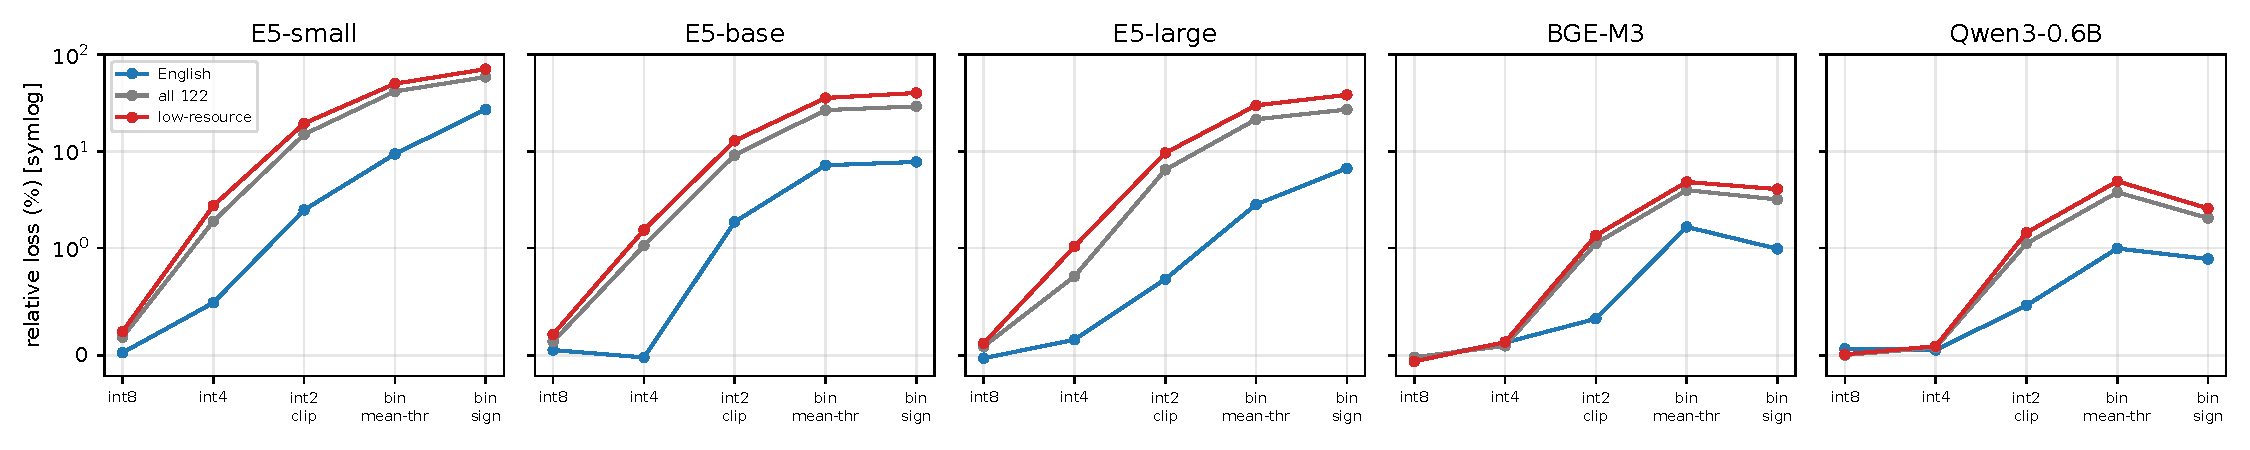
\includegraphics[width=\textwidth]{figs/fig2_loss_by_bits.pdf}
\caption{Relative loss by format for English, the mean over 122 languages and the mean over the 47 low-resource languages, per model. Symmetric-log vertical axis.}\label{fig:bits}\end{figure*}
\begin{figure}[t]\centering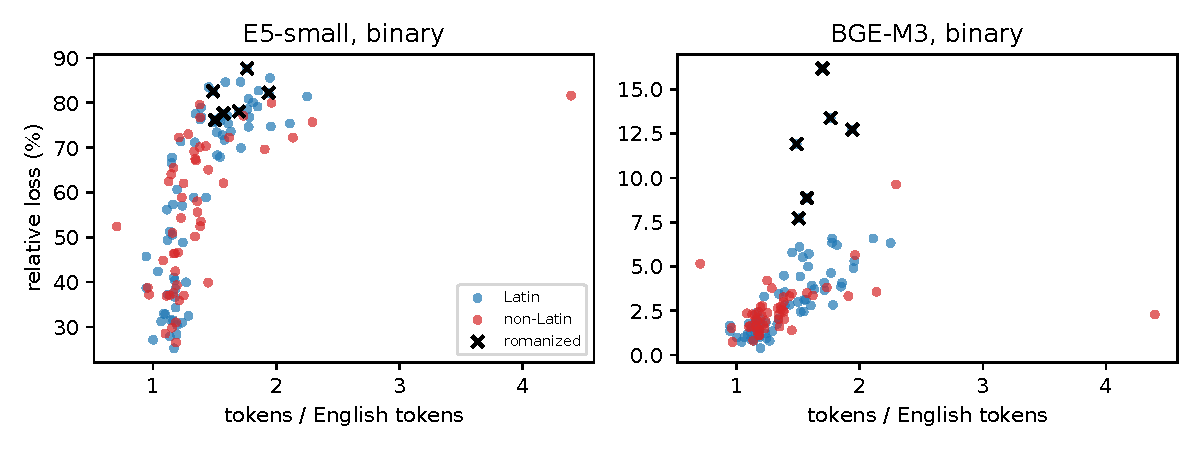
\includegraphics[width=\columnwidth]{figs/fig3_loss_vs_fertility.pdf}
\caption{Binary loss per language against tokenizer fertility for E5-small and BGE-M3; crosses are romanized variants. Fertility predicts the loss with much more scatter than the margin.}\label{fig:fert}\end{figure}
\begin{table}[t]\centering\footnotesize
\begin{tabular}{llrrrrr}
\toprule
 & & \multicolumn{5}{c}{bits per dimension needed} \\
model & retain & 1 & 2 & 4 & 8 & $>$8 \\
\midrule
E5-small & 99\% & -- & -- & 58 & 61 & 3 \\
 & 95\% & -- & 11 & 100 & 11 & -- \\
E5-base & 99\% & -- & -- & 82 & 37 & 3 \\
 & 95\% & -- & 45 & 75 & 1 & 1 \\
E5-large & 99\% & -- & 3 & 84 & 35 & -- \\
 & 95\% & 2 & 61 & 58 & 1 & -- \\
BGE-M3 & 99\% & 11 & 62 & 48 & 1 & -- \\
 & 95\% & 103 & 17 & 2 & -- & -- \\
Qwen3-0.6B & 99\% & 19 & 45 & 58 & -- & -- \\
 & 95\% & 119 & 2 & 1 & -- & -- \\
\bottomrule
\end{tabular}
\caption{Number of the 122 languages for which each bit width is the smallest that retains 99\% (or 95\%) of the language's float32 nDCG@10. int2 uses percentile clipping, 1 bit is the sign; English calibration. $>$8: not reached by int8.}\label{tab:bits}
\end{table}

\begin{table}[t]\centering\footnotesize
\resizebox{\columnwidth}{!}{\begin{tabular}{llrrrrrr}\toprule
 & & \multicolumn{2}{c}{margin} & \multicolumn{2}{c}{int2-clip loss} & \multicolumn{2}{c}{binary loss} \\
language & script & native & Latin & native & Latin & native & Latin \\ \midrule
Arabic & Arab & 0.033 & -0.022 & 4.2 & 18.6 & 21.5 & 66.3 \\
Bengali & Beng & 0.022 & -0.007 & 6.6 & 27.2 & 35.4 & 65.7 \\
Hindi & Deva & 0.028 & -0.001 & 5.8 & 21.7 & 26.0 & 59.9 \\
Nepali & Deva & 0.014 & -0.012 & 10.4 & 23.1 & 45.2 & 68.8 \\
Sinhala & Sinh & 0.013 & -0.017 & 9.9 & 39.2 & 46.8 & 79.9 \\
Urdu & Arab & 0.015 & -0.014 & 10.3 & 28.7 & 43.4 & 68.3 \\ \bottomrule
\end{tabular}}
\caption{Same language in its native script and romanized (E5-small and E5-base pooled): float32 margin and loss (\%). Identical content; only the script changes.}\label{tab:script}
\end{table}
\begin{figure*}[t]\centering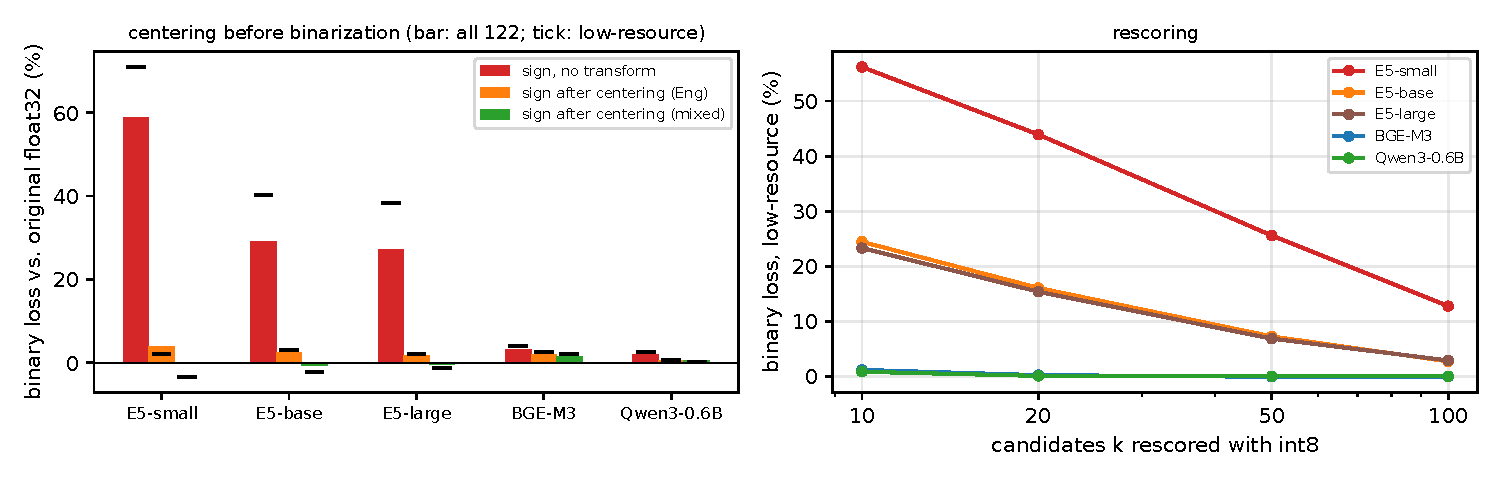
\includegraphics[width=0.85\textwidth]{figs/fig4_centring_rescoring.pdf}
\caption{Left: binary loss relative to the original float32 quality without a transform and after the centering transform fitted on English or on the mixed sample (bars: mean over 122 languages; ticks: low-resource mean). Right: binary loss on low-resource languages after rescoring $k$ candidates against an int8 corpus.}\label{fig:fix}\end{figure*}
\begin{table*}[t]\centering\footnotesize
\begin{tabular}{llrrrrr}
\toprule
scheme & languages & English & mixed (LOO) & Latin-only & target, 64 & target, all \\
\midrule
int2 & all 122 & 20.1 & 20.6 & 19.9 & 9.5 & 15.9 \\
 & low-res. & 27.3 & 27.7 & 26.8 & 12.6 & 20.6 \\
int2-clip & all 122 & 10.2 & 9.5 & 9.5 & 7.7 & 7.2 \\
 & low-res. & 14.0 & 13.0 & 13.1 & 10.4 & 9.8 \\
bin-mean-thr & all 122 & 29.9 & 27.9 & 27.8 & 23.4 & 23.3 \\
 & low-res. & 38.6 & 35.6 & 35.4 & 30.1 & 30.1 \\
\bottomrule
\end{tabular}
\caption{Loss (\%) by calibration source, E5 models pooled; 1388 vectors except ``target, 64''; LOO = leave-target-language-out.}\label{tab:calib}
\end{table*}
\begin{table*}[t]\centering\footnotesize
\begin{tabular}{lllrrrrr}
\toprule
model & scheme & languages & English & mixed (LOO) & Latin-only & target, 64 & target, all \\
\midrule
E5-small & int2 & all & 29.3 & 29.9 & 28.2 & 14.4 & 23.7 \\
 &  & low-res. & 37.9 & 38.2 & 35.9 & 18.0 & 29.1 \\
 & int2-clip & all & 15.0 & 13.4 & 13.9 & 11.8 & 11.2 \\
 &  & low-res. & 19.4 & 17.5 & 18.3 & 15.2 & 14.8 \\
 & bin-mean-thr & all & 41.7 & 39.9 & 40.0 & 34.8 & 34.6 \\
 &  & low-res. & 50.1 & 47.6 & 47.6 & 42.7 & 42.7 \\
\midrule
E5-base & int2 & all & 17.8 & 18.3 & 18.4 & 8.4 & 14.0 \\
 &  & low-res. & 24.6 & 25.5 & 25.6 & 11.6 & 18.8 \\
 & int2-clip & all & 9.1 & 8.8 & 8.6 & 6.6 & 6.2 \\
 &  & low-res. & 12.8 & 12.4 & 12.0 & 8.9 & 8.4 \\
 & bin-mean-thr & all & 26.7 & 24.2 & 24.0 & 20.2 & 20.2 \\
 &  & low-res. & 35.7 & 31.9 & 31.4 & 26.2 & 26.1 \\
\midrule
E5-large & int2 & all & 13.3 & 13.5 & 13.1 & 5.8 & 9.9 \\
 &  & low-res. & 19.4 & 19.4 & 18.8 & 8.2 & 13.8 \\
 & int2-clip & all & 6.4 & 6.2 & 6.0 & 4.7 & 4.2 \\
 &  & low-res. & 9.6 & 9.1 & 8.9 & 7.1 & 6.2 \\
 & bin-mean-thr & all & 21.5 & 19.5 & 19.4 & 15.2 & 15.2 \\
 &  & low-res. & 29.9 & 27.3 & 27.2 & 21.5 & 21.4 \\
\midrule
BGE-M3 & int2 & all & 2.7 & 2.8 & 2.7 & 1.5 & 2.6 \\
 &  & low-res. & 3.5 & 3.7 & 3.4 & 2.0 & 3.4 \\
 & int2-clip & all & 1.1 & 1.2 & 1.2 & 1.4 & 1.3 \\
 &  & low-res. & 1.3 & 1.4 & 1.4 & 1.9 & 1.6 \\
 & bin-mean-thr & all & 4.0 & 3.9 & 4.0 & 4.1 & 4.1 \\
 &  & low-res. & 4.8 & 4.8 & 4.8 & 5.3 & 5.3 \\
\midrule
Qwen3-0.6B & int2 & all & 2.3 & 2.4 & 2.3 & 1.2 & 2.2 \\
 &  & low-res. & 2.8 & 3.2 & 3.0 & 1.5 & 2.8 \\
 & int2-clip & all & 1.1 & 1.1 & 1.2 & 1.4 & 1.3 \\
 &  & low-res. & 1.4 & 1.5 & 1.6 & 1.9 & 1.8 \\
 & bin-mean-thr & all & 3.8 & 3.9 & 3.9 & 4.3 & 4.3 \\
 &  & low-res. & 4.9 & 5.1 & 5.3 & 5.8 & 5.7 \\
\bottomrule
\end{tabular}
\caption{Loss (\%) by calibration source for every model (1388 vectors except ``target, 64''; LOO = leave-target-language-out).}\label{tab:calib_full}
\end{table*}
\begin{table*}[t]\centering\footnotesize
\begin{tabular}{llrrrrrrr}
\toprule
model & transform (calib.) & nDCG$_{32}$ & $\bar{c}$ & margin & bin all & bin low & bin vs.\ $\mathrm{nDCG}_{32}'$ & int2-clip all \\
\midrule
E5-small & none & 0.692 & 0.79 & 0.010 & 58.8 & 70.9 & 58.8 & 15.0 \\
 & center (Eng) & 0.735 & 0.35 & 0.043 & 3.9 & 2.1 & 11.5 & -4.9 \\
 & center (mixed) & 0.741 & 0.25 & 0.049 & 0.0 & -3.3 & 9.2 & -7.3 \\
 & ZCA (Eng) & 0.576 & 0.55 & -0.004 & 38.6 & 46.8 & 24.6 & 26.7 \\
 & ZCA (mixed) & 0.733 & 0.14 & 0.058 & -0.6 & -7.2 & 8.9 & -8.2 \\
\midrule
E5-base & none & 0.736 & 0.78 & 0.016 & 29.2 & 40.2 & 29.2 & 9.1 \\
 & center (Eng) & 0.764 & 0.34 & 0.054 & 2.6 & 3.0 & 7.0 & -2.8 \\
 & center (mixed) & 0.774 & 0.27 & 0.063 & -0.6 & -2.3 & 5.7 & -4.9 \\
 & ZCA (Eng) & 0.503 & 0.58 & -0.014 & 48.3 & 62.9 & 21.7 & 40.3 \\
 & ZCA (mixed) & 0.735 & 0.20 & 0.054 & 6.2 & 3.7 & 7.5 & 0.5 \\
\midrule
E5-large & none & 0.785 & 0.77 & 0.021 & 27.1 & 38.4 & 27.1 & 6.4 \\
 & center (Eng) & 0.804 & 0.33 & 0.067 & 1.8 & 2.1 & 4.8 & -1.7 \\
 & center (mixed) & 0.811 & 0.26 & 0.076 & -0.4 & -1.2 & 3.8 & -3.2 \\
 & ZCA (Eng) & 0.522 & 0.60 & -0.010 & 48.1 & 61.0 & 20.0 & 40.9 \\
 & ZCA (mixed) & 0.761 & 0.19 & 0.061 & 8.4 & 7.8 & 6.0 & 4.1 \\
\midrule
BGE-M3 & none & 0.805 & 0.41 & 0.064 & 3.2 & 4.1 & 3.2 & 1.1 \\
 & center (Eng) & 0.808 & 0.18 & 0.092 & 1.9 & 2.6 & 2.4 & 0.3 \\
 & center (mixed) & 0.809 & 0.15 & 0.094 & 1.6 & 2.1 & 2.2 & 0.0 \\
 & ZCA (Eng) & 0.732 & 0.17 & 0.058 & 15.4 & 18.3 & 6.2 & 11.5 \\
 & ZCA (mixed) & 0.769 & 0.07 & 0.077 & 8.7 & 9.7 & 4.1 & 5.8 \\
\midrule
Qwen3-0.6B & none & 0.708 & 0.32 & 0.055 & 2.0 & 2.6 & 2.0 & 1.1 \\
 & center (Eng) & 0.713 & 0.13 & 0.071 & 0.6 & 0.7 & 1.5 & -0.3 \\
 & center (mixed) & 0.713 & 0.11 & 0.071 & 0.5 & 0.3 & 1.5 & -0.4 \\
 & ZCA (Eng) & 0.671 & 0.20 & 0.044 & 8.7 & 9.4 & 3.7 & 6.0 \\
 & ZCA (mixed) & 0.715 & 0.09 & 0.072 & 1.3 & 0.8 & 2.8 & -0.9 \\
\bottomrule
\end{tabular}
\caption{Centering and whitening before compression. nDCG$_{32}$: float32 quality after the transform (mean over 122 languages); $\bar{c}$: mean passage cosine; margin: mean float32 margin. Losses are relative to the \emph{original} float32 quality, except the column marked vs.\ nDCG$_{32}'$, which is relative to the transformed float32 quality. Negative values are gains over the original float32 baseline.}\label{tab:whiten}
\end{table*}
\begin{table*}[t]\centering\footnotesize
\begin{tabular}{llrrrrrrrrrrrr}
\toprule
model & index & \multicolumn{3}{c}{$k=10$} & \multicolumn{3}{c}{$k=20$} & \multicolumn{3}{c}{$k=50$} & \multicolumn{3}{c}{$k=100$} \\
 & & Eng & all & low & Eng & all & low & Eng & all & low & Eng & all & low \\
\midrule
E5-small & binary & 13.1 & 43.6 & 56.2 & 7.9 & 32.8 & 43.9 & 3.3 & 18.4 & 25.6 & 1.4 & 9.0 & 12.8 \\
 & int2-clip & 0.2 & 6.3 & 8.5 & 0.0 & 2.8 & 3.8 & 0.1 & 0.6 & 0.8 & 0.0 & 0.3 & 0.3 \\
E5-base & binary & 2.3 & 16.6 & 24.4 & 1.3 & 10.5 & 16.1 & 0.2 & 4.6 & 7.3 & 0.2 & 1.7 & 2.7 \\
 & int2-clip & 0.1 & 3.3 & 5.0 & 0.0 & 1.3 & 1.9 & 0.0 & 0.3 & 0.4 & 0.0 & 0.1 & 0.2 \\
E5-large & binary & 2.7 & 15.4 & 23.3 & 1.2 & 9.9 & 15.4 & 0.4 & 4.3 & 6.9 & 0.1 & 1.7 & 2.9 \\
 & int2-clip & -0.1 & 2.2 & 3.4 & -0.1 & 0.7 & 1.1 & 0.0 & 0.2 & 0.4 & 0.0 & 0.2 & 0.3 \\
BGE-M3 & binary & 0.0 & 0.9 & 1.2 & 0.0 & 0.2 & 0.2 & 0.0 & 0.0 & -0.1 & 0.0 & 0.0 & -0.1 \\
 & int2-clip & -0.1 & 0.2 & 0.3 & 0.0 & 0.0 & 0.0 & 0.0 & 0.0 & -0.1 & 0.0 & 0.0 & -0.1 \\
Qwen3-0.6B & binary & 0.1 & 0.6 & 0.8 & 0.1 & 0.1 & 0.1 & 0.1 & 0.0 & 0.0 & 0.1 & 0.0 & 0.0 \\
 & int2-clip & 0.2 & 0.3 & 0.4 & 0.1 & 0.0 & 0.0 & 0.1 & 0.0 & 0.0 & 0.1 & 0.0 & 0.0 \\
\bottomrule
\end{tabular}
\caption{Loss (\%) after retrieving $k$ candidates with the compressed index and rescoring them with the float32 query against an int8 corpus. Rescoring with the float32 corpus differs by at most 0.2 points. English calibration.}\label{tab:rescore}
\end{table*}

\section{Mechanism and robustness analyses}\label{app:mech}
Tables~\ref{tab:graded} and~\ref{tab:flip} measure the score perturbation caused by sign binarization for E5-small, with the English calibration mean removed in steps and per query. Table~\ref{tab:heldout} repeats the calibration comparison with a calibration set that shares no content with Belebele. Table~\ref{tab:dist} reports the distribution of the binary loss and the low-resource gap under a second definition of low-resource.
\begin{table}[t]\centering\footnotesize
\resizebox{\columnwidth}{!}{\begin{tabular}{rrrrrrr}
\toprule
$\alpha$ & $\bar{c}$ & margin & perturb. & float32 & loss & loss own \\
\midrule
0.00 & 0.79 & 0.010 & 0.024 & 0.692 & 58.8 & 58.8 \\
0.25 & 0.70 & 0.016 & 0.027 & 0.699 & 42.1 & 42.7 \\
0.50 & 0.56 & 0.025 & 0.032 & 0.712 & 23.5 & 25.9 \\
0.75 & 0.41 & 0.037 & 0.037 & 0.728 & 9.1 & 14.8 \\
1.00 & 0.35 & 0.043 & 0.038 & 0.735 & 3.9 & 11.5 \\
\bottomrule
\end{tabular}}
\caption{Graded centering, E5-small, mean over 122 languages: documents and queries are shifted by $-\alpha\vmu$ ($\vmu$: English calibration mean) and re-normalized. perturb.: standard deviation over documents of the change in score caused by sign binarization (compressed scores rescaled per query to the float32 scale); float32: nDCG@10 after the shift; loss: binary loss (\%) relative to the original float32 quality; loss own: relative to the float32 quality after the shift.}\label{tab:graded}
\end{table}

\begin{table}[t]\centering\footnotesize
\begin{tabular}{lrrrr}
\toprule
 & \multicolumn{2}{c}{not centered} & \multicolumn{2}{c}{centered} \\
margin / perturb. & lost & queries & lost & queries \\
\midrule
$<0.25$ & 94\% & 7{,}825 & 68\% & 3{,}533 \\
0.25--0.5 & 90\% & 7{,}816 & 60\% & 3{,}530 \\
0.5--1 & 83\% & 14{,}683 & 47\% & 7{,}332 \\
1--2 & 61\% & 22{,}165 & 24\% & 14{,}557 \\
$>2$ & 21\% & 13{,}479 & 2\% & 42{,}296 \\
\bottomrule
\end{tabular}
\caption{Share of queries ranked first at float32 that lose the first rank under sign binarization, by the ratio of the query's float32 margin to the perturbation of its scores (E5-small, all 122 languages pooled).}\label{tab:flip}
\end{table}

\begin{table}[t]\centering\footnotesize
\resizebox{\columnwidth}{!}{\begin{tabular}{llrrr}
\toprule
format & calibration & English & all & low \\
\midrule
int2 & Belebele English & 6.6 & 29.3 & 37.9 \\
 & Wikipedia English & 6.3 $\pm$ 0.4 & 30.4 $\pm$ 0.4 & 38.8 $\pm$ 0.7 \\
 & Belebele mixed & 6.7 $\pm$ 0.8 & 29.7 $\pm$ 0.2 & 38.2 $\pm$ 0.3 \\
\midrule
int2-clip & Belebele English & 2.5 & 15.0 & 19.4 \\
 & Wikipedia English & 2.2 $\pm$ 0.1 & 15.0 $\pm$ 0.1 & 19.8 $\pm$ 0.2 \\
 & Belebele mixed & 2.9 $\pm$ 0.2 & 13.5 $\pm$ 0.2 & 17.7 $\pm$ 0.3 \\
\midrule
bin-mean-thr & Belebele English & 9.4 & 41.7 & 50.1 \\
 & Wikipedia English & 10.7 $\pm$ 0.2 & 42.4 $\pm$ 0.2 & 51.8 $\pm$ 0.3 \\
 & Belebele mixed & 12.1 $\pm$ 0.6 & 39.7 $\pm$ 0.0 & 47.3 $\pm$ 0.2 \\
\midrule
centering + sign & Belebele English & 3.1 & 3.9 & 2.1 \\
 & Wikipedia English & 2.9 $\pm$ 0.1 & 5.6 $\pm$ 0.1 & 5.1 $\pm$ 0.2 \\
 & Belebele mixed & 3.0 $\pm$ 0.2 & 0.0 $\pm$ 0.2 & -3.3 $\pm$ 0.3 \\
\bottomrule
\end{tabular}}
\caption{Calibration without content overlap, E5-small: loss (\%) with the Belebele English evaluation data as calibration set (one set), with 1388 English Wikipedia passages that share no content with Belebele (five draws), and with the mixed leave-target-out Belebele sample (five draws); mean $\pm$ standard deviation over draws.}\label{tab:heldout}
\end{table}

\begin{table*}[t]\centering\footnotesize
\begin{tabular}{lrrrrlrrr}
\toprule
 & \multicolumn{5}{c}{all 122 languages} & \multicolumn{3}{c}{low-resource gap} \\
\cmidrule(lr){2-6}\cmidrule(lr){7-9}
model & mean & median & 90th pct. & worst & worst language & class 0--1 & fewest articles & rest \\
\midrule
E5-small & 58.8 & 62.2 & 80.0 & 87.7 & Sinhala (romanized) & 70.9 & 73.6 & 49.6 \\
E5-base & 29.2 & 27.9 & 51.1 & 72.2 & Sinhala (romanized) & 40.2 & 42.5 & 20.9 \\
E5-large & 27.1 & 24.5 & 52.1 & 75.6 & Sinhala (romanized) & 38.4 & 41.6 & 18.0 \\
BGE-M3 & 3.2 & 2.4 & 6.1 & 16.2 & Urdu (romanized) & 4.1 & 4.3 & 2.5 \\
Qwen3-0.6B & 2.0 & 1.9 & 3.3 & 7.6 & Tigrinya & 2.6 & 2.8 & 1.5 \\
\bottomrule
\end{tabular}
\caption{Distribution of the binary loss (\%) over the 122 languages, and the low-resource gap under two definitions: resource classes 0--1 \citep{joshi2020state}, and the 47 languages with the fewest Wikipedia articles (rest: the other languages with a Wikipedia count).}\label{tab:dist}
\end{table*}


\onecolumn
\section{Per-language results}\label{app:perlang}
Table~\ref{tab:perlang} lists, for every language, the loss under binary and int2-clip storage for each model. Results for all formats, calibration sources, transforms and query modes, with margins, fertility and geometry statistics, are in the released CSV files.
\begin{small}
\begin{longtable}{llrrrrrrrrrrr}
\caption{Per-language relative loss (\%) under binarization (bin) and int2-clip (int2) for every model; J = Joshi class.}\label{tab:perlang}\\
\toprule
language & script & J & \multicolumn{2}{c}{E5-small} & \multicolumn{2}{c}{E5-base} & \multicolumn{2}{c}{E5-large} & \multicolumn{2}{c}{BGE-M3} & \multicolumn{2}{c}{Qwen3-0.6B} \\
 & & & bin & int2 & bin & int2 & bin & int2 & bin & int2 & bin & int2 \\
\midrule
\endfirsthead
\toprule
language & script & J & \multicolumn{2}{c}{E5-small} & \multicolumn{2}{c}{E5-base} & \multicolumn{2}{c}{E5-large} & \multicolumn{2}{c}{BGE-M3} & \multicolumn{2}{c}{Qwen3-0.6B} \\
 & & & bin & int2 & bin & int2 & bin & int2 & bin & int2 & bin & int2 \\
\midrule
\endhead
\bottomrule
\endfoot
Mesopotamian Arabic & Arab & -- & 47 & 8 & 19 & 4 & 14 & 3 & 2 & 0 & 1 & 1 \\
Afrikaans & Latn & 3 & 61 & 12 & 22 & 4 & 24 & 3 & 2 & 1 & 2 & 1 \\
Tosk Albanian & Latn & 1 & 59 & 14 & 27 & 7 & 17 & 3 & 2 & 0 & 2 & 1 \\
Amharic & Ethi & 2 & 69 & 22 & 36 & 11 & 36 & 7 & 3 & 1 & 4 & 2 \\
North Levantine Arabic & Arab & -- & 51 & 10 & 16 & 4 & 18 & 3 & 2 & 1 & 0 & 0 \\
Standard Arabic & Arab & 5 & 31 & 5 & 12 & 3 & 6 & 2 & 1 & 0 & 1 & 0 \\
Arabic (romanized) & Latn & 5 & 82 & 21 & 50 & 16 & 65 & 14 & 13 & 3 & 3 & 1 \\
Najdi Arabic & Arab & -- & 39 & 9 & 17 & 4 & 10 & 2 & 3 & 1 & 1 & 1 \\
Moroccan Arabic & Arab & -- & 62 & 22 & 30 & 7 & 39 & 7 & 4 & 2 & 2 & 1 \\
Egyptian Arabic & Arab & 3 & 46 & 11 & 25 & 6 & 20 & 4 & 2 & 0 & 1 & 0 \\
Assamese & Beng & 1 & 70 & 21 & 39 & 9 & 35 & 8 & 3 & 2 & 3 & 1 \\
North Azerbaijani & Latn & 1 & 68 & 11 & 27 & 7 & 25 & 5 & 2 & 0 & 1 & 1 \\
Bambara & Latn & 1 & 80 & 19 & 45 & 13 & 47 & 15 & 6 & 2 & 1 & 1 \\
Bengali & Beng & 3 & 54 & 8 & 17 & 5 & 19 & 4 & 2 & 1 & 2 & 1 \\
Bengali (romanized) & Latn & 3 & 78 & 35 & 54 & 19 & 50 & 15 & 9 & 2 & 3 & 2 \\
Tibetan & Tibt & 1 & 52 & 14 & 66 & 15 & 52 & 16 & 5 & 2 & 6 & 5 \\
Bulgarian & Cyrl & 3 & 30 & 6 & 10 & 3 & 7 & 2 & 2 & 0 & 1 & 1 \\
Catalan & Latn & 4 & 40 & 7 & 13 & 2 & 7 & 2 & 1 & 0 & 1 & 0 \\
Cebuano & Latn & 3 & 68 & 19 & 33 & 10 & 34 & 7 & 2 & 0 & 1 & 1 \\
Czech & Latn & 4 & 31 & 4 & 8 & 2 & 6 & 2 & 2 & 0 & 1 & 1 \\
Central Kurdish & Arab & 1 & 76 & 25 & 53 & 20 & 49 & 15 & 10 & 2 & 3 & 2 \\
Danish & Latn & 3 & 33 & 5 & 10 & 3 & 6 & 2 & 2 & 1 & 1 & 1 \\
German & Latn & 5 & 25 & 4 & 10 & 2 & 6 & 1 & 1 & 0 & 0 & 0 \\
Greek & Grek & 3 & 40 & 8 & 14 & 4 & 6 & 2 & 1 & 0 & 1 & 0 \\
English & Latn & 5 & 27 & 2 & 8 & 2 & 7 & 1 & 1 & 0 & 1 & 0 \\
Estonian & Latn & 3 & 37 & 8 & 14 & 4 & 10 & 2 & 2 & 0 & 3 & 0 \\
Basque & Latn & 4 & 51 & 12 & 18 & 4 & 11 & 3 & 2 & 0 & 3 & 2 \\
Finnish & Latn & 4 & 31 & 5 & 9 & 3 & 5 & 1 & 1 & 1 & 2 & 1 \\
French & Latn & 5 & 32 & 6 & 11 & 2 & 6 & 1 & 1 & 0 & 1 & 0 \\
Nigerian Fulfulde & Latn & 0 & 84 & 27 & 51 & 22 & 61 & 17 & 6 & 2 & 3 & 2 \\
West Central Oromo & Latn & 1 & 81 & 30 & 51 & 24 & 54 & 17 & 6 & 2 & 5 & 1 \\
Guarani & Latn & 1 & 85 & 23 & 51 & 14 & 49 & 17 & 4 & 1 & 1 & 1 \\
Gujarati & Gujr & 1 & 70 & 15 & 39 & 10 & 32 & 6 & 3 & 2 & 2 & 1 \\
Haitian Creole & Latn & 2 & 79 & 21 & 45 & 14 & 47 & 8 & 3 & 2 & 3 & 2 \\
Hausa & Latn & 2 & 77 & 19 & 34 & 12 & 35 & 12 & 4 & 1 & 3 & 2 \\
Hebrew & Hebr & 3 & 37 & 7 & 15 & 5 & 8 & 2 & 1 & 0 & 2 & 1 \\
Hindi & Deva & 4 & 37 & 7 & 15 & 5 & 11 & 2 & 2 & 1 & 1 & 0 \\
Hindi (romanized) & Latn & 4 & 76 & 25 & 44 & 19 & 47 & 13 & 8 & 2 & 1 & 2 \\
Croatian & Latn & 4 & 56 & 9 & 12 & 4 & 9 & 2 & 1 & 1 & 2 & 0 \\
Hungarian & Latn & 4 & 39 & 8 & 11 & 2 & 6 & 1 & 1 & 1 & 1 & 0 \\
Armenian & Armn & 1 & 70 & 22 & 37 & 16 & 40 & 9 & 3 & 1 & 2 & 2 \\
Igbo & Latn & 1 & 75 & 27 & 51 & 17 & 43 & 12 & 7 & 2 & 3 & 1 \\
Ilocano & Latn & 1 & 77 & 19 & 37 & 11 & 35 & 10 & 3 & 1 & 1 & 1 \\
Indonesian & Latn & 3 & 39 & 6 & 7 & 2 & 7 & 2 & 1 & 0 & 1 & 1 \\
Icelandic & Latn & 2 & 57 & 15 & 24 & 8 & 13 & 4 & 2 & 1 & 2 & 1 \\
Italian & Latn & 4 & 30 & 4 & 9 & 3 & 8 & 2 & 0 & 0 & 0 & 0 \\
Javanese & Latn & 1 & 67 & 13 & 33 & 8 & 31 & 6 & 2 & 1 & 3 & 2 \\
Japanese & Jpan & 5 & 37 & 6 & 10 & 2 & 7 & 2 & 2 & 1 & 1 & 1 \\
Jingpho & Latn & 0 & 86 & 30 & 56 & 12 & 57 & 14 & 5 & 1 & 2 & 1 \\
Kannada & Knda & 1 & 56 & 12 & 25 & 7 & 18 & 4 & 3 & 0 & 1 & 1 \\
Georgian & Geor & 3 & 67 & 22 & 35 & 12 & 25 & 5 & 2 & 1 & 3 & 1 \\
Kazakh & Cyrl & 3 & 64 & 16 & 32 & 9 & 31 & 7 & 2 & 1 & 2 & 1 \\
Kabuverdianu & Latn & -- & 78 & 26 & 53 & 16 & 42 & 7 & 3 & 3 & 2 & 1 \\
Halh Mongolian & Cyrl & 1 & 72 & 17 & 38 & 15 & 41 & 9 & 3 & 1 & 3 & 2 \\
Khmer & Khmr & 1 & 72 & 23 & 47 & 14 & 46 & 13 & 3 & 1 & 3 & 2 \\
Kinyarwanda & Latn & 1 & 70 & 21 & 34 & 8 & 34 & 5 & 4 & 1 & 2 & 2 \\
Kyrgyz & Cyrl & 1 & 66 & 17 & 29 & 11 & 28 & 6 & 2 & 1 & 3 & 1 \\
Korean & Hang & 4 & 38 & 6 & 11 & 3 & 7 & 2 & 2 & 0 & 1 & 1 \\
Lao & Laoo & 2 & 77 & 24 & 35 & 21 & 35 & 12 & 3 & 1 & 3 & 3 \\
Lingala & Latn & 1 & 73 & 15 & 51 & 13 & 37 & 12 & 4 & 1 & 4 & 1 \\
Lithuanian & Latn & 3 & 41 & 9 & 13 & 3 & 7 & 2 & 1 & 1 & 2 & 1 \\
Ganda & Latn & 1 & 77 & 17 & 48 & 13 & 57 & 9 & 6 & 3 & 2 & 1 \\
Luo & Latn & -- & 76 & 21 & 47 & 17 & 42 & 10 & 6 & 1 & 2 & 1 \\
Standard Latvian & Latn & 3 & 49 & 13 & 16 & 4 & 8 & 2 & 1 & 0 & 2 & 1 \\
Malayalam & Mlym & 1 & 52 & 9 & 24 & 5 & 16 & 2 & 2 & 1 & 2 & 1 \\
Marathi & Deva & 2 & 54 & 11 & 22 & 8 & 16 & 2 & 2 & 0 & 2 & 1 \\
Macedonian & Cyrl & 1 & 46 & 11 & 12 & 4 & 8 & 2 & 1 & 0 & 2 & 1 \\
Maltese & Latn & 2 & 75 & 16 & 35 & 8 & 38 & 5 & 5 & 2 & 2 & 2 \\
Maori & Latn & 1 & 83 & 22 & 48 & 18 & 60 & 13 & 4 & 2 & 3 & 0 \\
Burmese & Mymr & 1 & 77 & 25 & 37 & 13 & 33 & 8 & 4 & 1 & 1 & 1 \\
Dutch & Latn & 4 & 28 & 5 & 11 & 2 & 6 & 1 & 1 & 0 & 1 & 0 \\
Norwegian Bokmal & Latn & 1 & 31 & 4 & 11 & 3 & 6 & 2 & 1 & 0 & 1 & 1 \\
Nepali & Deva & 1 & 62 & 13 & 28 & 8 & 21 & 5 & 2 & 1 & 3 & 1 \\
Nepali (romanized) & Latn & 1 & 83 & 23 & 55 & 24 & 61 & 16 & 12 & 4 & 3 & 2 \\
Northern Sotho & Latn & 1 & 79 & 18 & 47 & 14 & 42 & 13 & 5 & 2 & 1 & 0 \\
Nyanja & Latn & 1 & 72 & 23 & 42 & 11 & 42 & 10 & 5 & 1 & 3 & 2 \\
Odia & Orya & 1 & 65 & 14 & 27 & 8 & 21 & 3 & 3 & 1 & 2 & 2 \\
Eastern Panjabi & Guru & -- & 62 & 18 & 32 & 11 & 26 & 4 & 4 & 1 & 2 & 1 \\
Southern Pashto & Arab & 1 & 80 & 21 & 44 & 11 & 42 & 7 & 3 & 1 & 4 & 3 \\
Western Persian & Arab & 4 & 29 & 5 & 10 & 3 & 7 & 2 & 2 & 1 & 1 & 1 \\
Plateau Malagasy & Latn & 1 & 73 & 19 & 39 & 9 & 32 & 8 & 3 & 1 & 4 & 2 \\
Polish & Latn & 4 & 34 & 6 & 10 & 4 & 7 & 2 & 1 & 1 & 1 & 1 \\
Portuguese & Latn & 4 & 49 & 9 & 15 & 4 & 10 & 3 & 1 & 1 & 1 & 0 \\
Romanian & Latn & 3 & 31 & 5 & 8 & 2 & 6 & 1 & 1 & 1 & 1 & 0 \\
Russian & Cyrl & 4 & 27 & 5 & 8 & 2 & 6 & 1 & 1 & 1 & 0 & 0 \\
Shan & Mymr & 0 & 82 & 39 & 49 & 19 & 57 & 20 & 2 & 0 & 3 & -1 \\
Sinhala (romanized) & Latn & 0 & 88 & 41 & 72 & 37 & 76 & 18 & 13 & 6 & 6 & 3 \\
Sinhala & Sinh & 0 & 67 & 12 & 27 & 8 & 22 & 5 & 2 & 0 & 3 & 4 \\
Slovak & Latn & 3 & 40 & 7 & 9 & 2 & 6 & 2 & 1 & 0 & 1 & 1 \\
Slovenian & Latn & 3 & 51 & 8 & 14 & 3 & 8 & 3 & 1 & 0 & 2 & 1 \\
Shona & Latn & 1 & 74 & 25 & 40 & 13 & 42 & 8 & 4 & 1 & 2 & 1 \\
Sindhi & Arab & 1 & 73 & 23 & 39 & 17 & 35 & 8 & 4 & 1 & 2 & 2 \\
Somali & Latn & 1 & 76 & 29 & 44 & 16 & 49 & 15 & 4 & 2 & 3 & 1 \\
Southern Sotho & Latn & 1 & 75 & 18 & 47 & 14 & 41 & 11 & 7 & 2 & 3 & 2 \\
Spanish & Latn & 5 & 28 & 5 & 8 & 2 & 5 & 1 & 2 & 1 & 0 & 0 \\
Serbian & Cyrl & 4 & 42 & 9 & 11 & 3 & 8 & 2 & 1 & 1 & 2 & 1 \\
Swati & Latn & 1 & 75 & 19 & 45 & 12 & 51 & 13 & 4 & 1 & 3 & 2 \\
Sundanese & Latn & 1 & 71 & 17 & 41 & 12 & 27 & 5 & 3 & 1 & 2 & 0 \\
Swedish & Latn & 4 & 33 & 5 & 10 & 3 & 5 & 2 & 1 & 1 & 1 & 1 \\
Swahili & Latn & 2 & 57 & 12 & 19 & 4 & 17 & 4 & 2 & 1 & 2 & 2 \\
Tamil & Taml & 3 & 58 & 11 & 23 & 6 & 17 & 3 & 3 & 0 & 2 & 1 \\
Telugu & Telu & 1 & 50 & 11 & 21 & 6 & 23 & 4 & 2 & 1 & 2 & 1 \\
Tajik & Cyrl & 1 & 72 & 14 & 41 & 18 & 41 & 12 & 4 & 1 & 2 & 1 \\
Tagalog & Latn & 3 & 59 & 12 & 24 & 7 & 19 & 4 & 3 & 1 & 1 & 0 \\
Thai & Thai & 3 & 45 & 10 & 16 & 4 & 9 & 2 & 2 & 1 & 1 & 0 \\
Tigrinya & Ethi & 2 & 80 & 23 & 49 & 24 & 47 & 14 & 6 & 3 & 8 & 1 \\
Tswana & Latn & 2 & 79 & 17 & 48 & 12 & 51 & 9 & 4 & 2 & 1 & 2 \\
Tsonga & Latn & 1 & 77 & 17 & 45 & 12 & 45 & 10 & 3 & 1 & 2 & 1 \\
Turkish & Latn & 4 & 42 & 6 & 8 & 3 & 8 & 2 & 1 & 0 & 2 & 0 \\
Ukrainian & Cyrl & 3 & 36 & 5 & 9 & 3 & 6 & 1 & 2 & 1 & 1 & 0 \\
Urdu & Arab & 3 & 59 & 13 & 28 & 7 & 19 & 5 & 2 & 1 & 2 & 1 \\
Urdu (romanized) & Latn & 3 & 78 & 34 & 58 & 23 & 65 & 16 & 16 & 6 & 2 & 2 \\
Northern Uzbek & Latn & 3 & 71 & 18 & 33 & 12 & 26 & 6 & 2 & 1 & 2 & 2 \\
Vietnamese & Latn & 4 & 37 & 8 & 8 & 2 & 6 & 2 & 1 & 0 & 0 & 0 \\
Waray & Latn & 1 & 68 & 15 & 28 & 9 & 29 & 6 & 2 & 0 & 1 & 1 \\
Wolof & Latn & 2 & 85 & 25 & 56 & 17 & 61 & 14 & 6 & 3 & 2 & 1 \\
Xhosa & Latn & 2 & 76 & 24 & 40 & 11 & 41 & 9 & 3 & 2 & 3 & 2 \\
Yoruba & Latn & 2 & 81 & 26 & 46 & 11 & 53 & 8 & 6 & 2 & 3 & 2 \\
Chinese (Simplified) & Hans & 5 & 37 & 8 & 12 & 4 & 18 & 5 & 1 & 0 & 0 & 0 \\
Chinese (Traditional) & Hant & 5 & 39 & 7 & 11 & 3 & 24 & 6 & 2 & 0 & 0 & 0 \\
Standard Malay & Latn & 3 & 46 & 6 & 11 & 3 & 11 & 1 & 2 & 0 & 0 & 1 \\
Zulu & Latn & 2 & 76 & 25 & 47 & 10 & 45 & 8 & 3 & 1 & 4 & 2 \\
\end{longtable}
\end{small}

\end{document}
